\batchmode
\makeatletter
\def\input@path{{\string"/Users/Tom/Documents/lyx/Materials for lyx workshop/presentation/\string"/}}
\makeatother
\documentclass[11pt,american]{article}
\usepackage[T1]{fontenc}
\usepackage[latin9]{inputenc}
\usepackage[letterpaper]{geometry}
\geometry{verbose,tmargin=1in,bmargin=1in,lmargin=1in,rmargin=1in,footskip=1cm}
\usepackage{amsmath}
\usepackage{amssymb}
\usepackage{graphicx}
\usepackage{setspace}
\doublespacing

\makeatletter

%%%%%%%%%%%%%%%%%%%%%%%%%%%%%% LyX specific LaTeX commands.
%% Because html converters don't know tabularnewline
\providecommand{\tabularnewline}{\\}

%%%%%%%%%%%%%%%%%%%%%%%%%%%%%% Textclass specific LaTeX commands.

%%%%%%%%%%%%%%%%%%%%%%%%%%%%%% User specified LaTeX commands.
\makeatother
\usepackage{graphicx}
\usepackage{lineno,setspace}
%\linenumbers
\usepackage[small,compact]{titlesec}
\usepackage[small,it]{caption}
%\addtolength{\textfloatsep}{-20mm}
%\doublespace
\addtolength{\belowcaptionskip}{-3mm}
\addtolength{\abovecaptionskip}{-3mm}
\usepackage{enumitem} % load the package
\usepackage{bm}
\usepackage{calc}
\usepackage{rotating}

\DeclareMathOperator{\dbin}{binomial}
\DeclareMathOperator{\dpois}{Poisson}
\DeclareMathOperator{\dnorm}{normal}
\DeclareMathOperator{\dlnorm}{lognormal}
\DeclareMathOperator{\dgamma}{gamma}
\DeclareMathOperator{\dunif}{uniform}
\DeclareMathOperator{\dmultinom}{multinomial}
\DeclareMathOperator{\dbeta}{beta}
\DeclareMathOperator{\ddirch}{Dirichlet}
\DeclareMathOperator{\dbern}{Bernoulli}



\addtolength{\intextsep}{-3mm}

\usepackage{fancyheadings}
\usepackage{url}
\usepackage[tablesfirst,notablist]{endfloat}

\makeatother

\usepackage{babel}
\usepackage{Sweave}
\begin{document}

\title{Sources of environmental conflict}


\author{N. T. Hobbs}
\maketitle
\begin{abstract}
This paper summarizes ten years of research on social and environmental....blah
blah blah
\end{abstract}

\section{Introduction}

Here we lay out out paper...

\begin{figure}
\center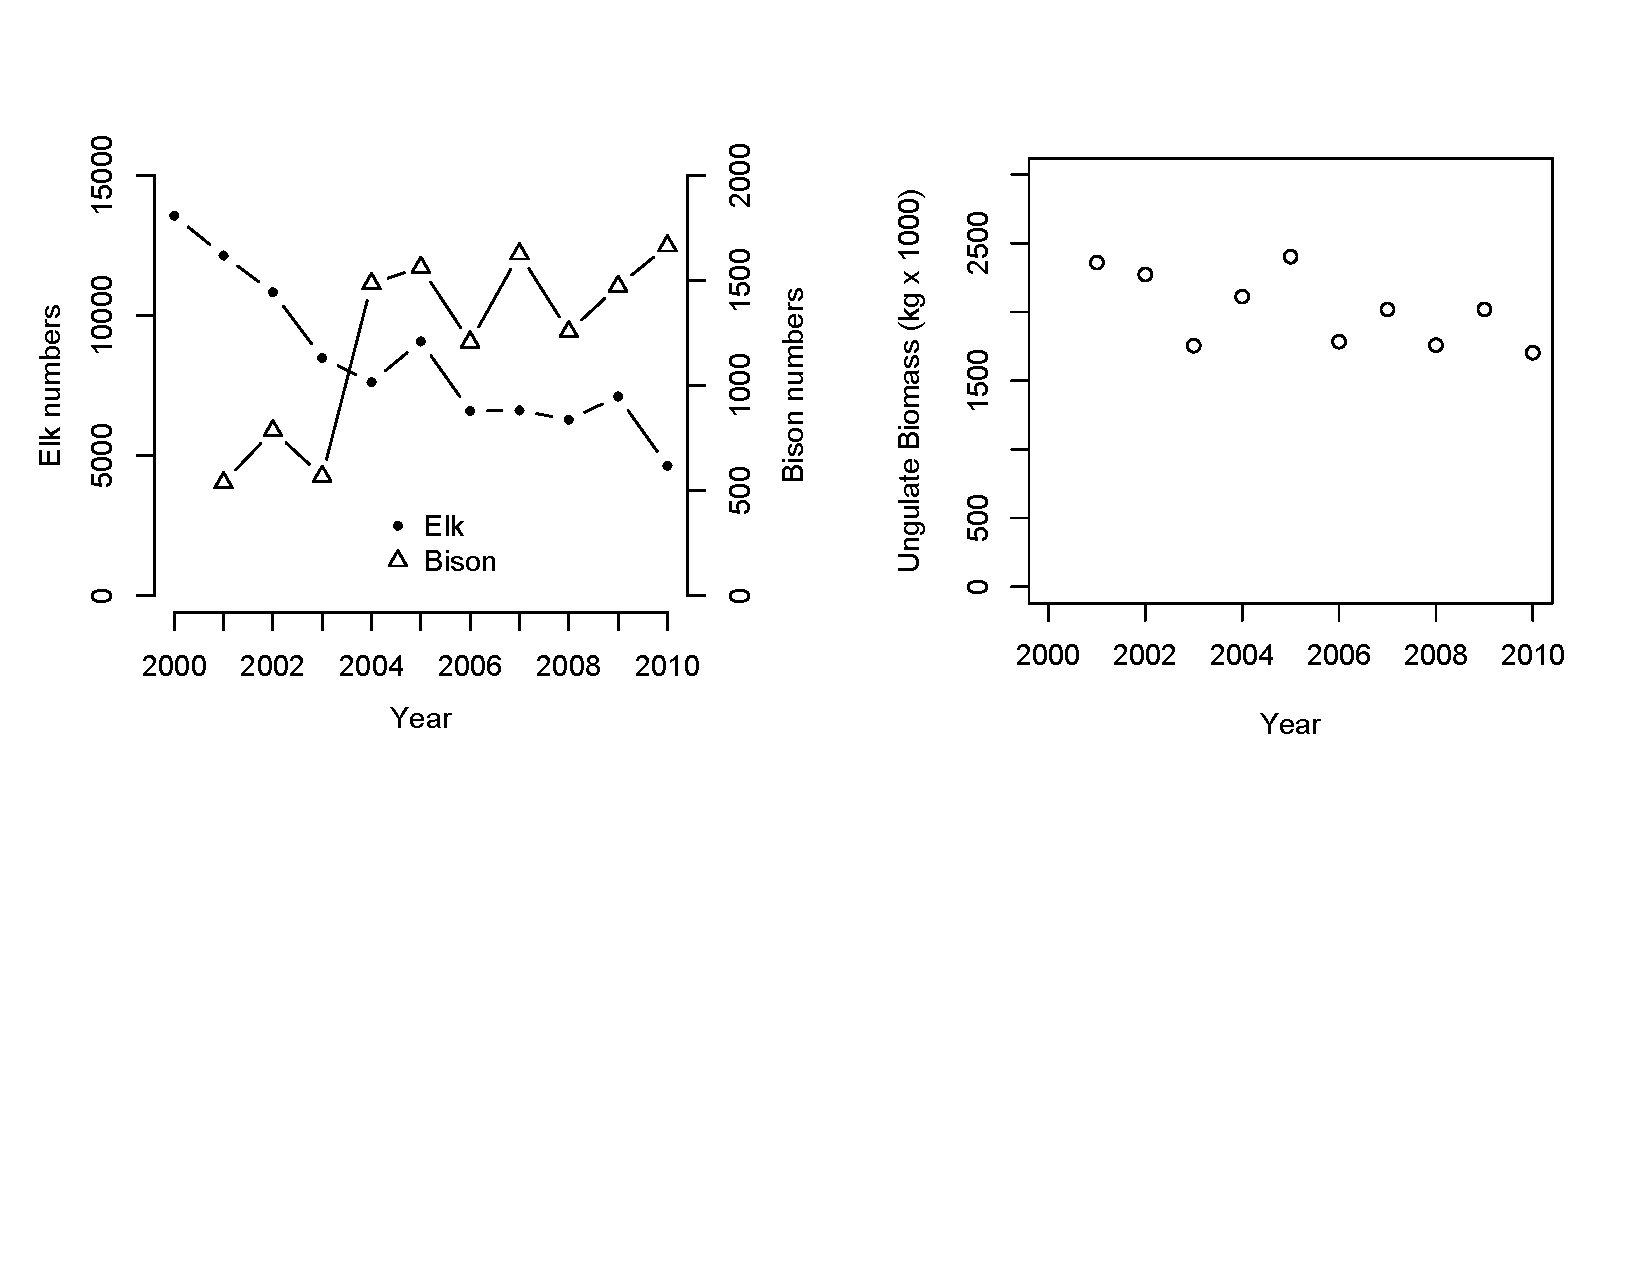
\includegraphics[width=5in]{47_Users_Tom_Documents_lyx_Materials_for_lyx_wo___LyX-templates1_NSF_Proposal_biomass_numbers.pdf}\caption{This is an example of a figure.}


\end{figure}


\begin{table}


\caption{Here is a table for our stunning paper}


\center%
\begin{tabular}{|c|c|c|c|c|}
\hline 
 &
Mean &
SD &
2.5\% CL &
97.5\% CL\tabularnewline
\hline 
\hline 
Intercept &
0.35 &
0.0172 &
0.317 &
0.384\tabularnewline
\hline 
Lynx &
-0.00784 &
0.00315 &
-0.014 &
-0.00165\tabularnewline
\hline 
Wolverine &
-0.0149 &
0.00409 &
-0.0229 &
-0.00684\tabularnewline
\hline 
Latitude &
-0.000591 &
4.43E-05 &
-0.000678 &
-0.000504\tabularnewline
\hline 
Reindeer Density &
-0.0229 &
0.0074 &
-0.0374 &
-0.00845\tabularnewline
\hline 
NAO &
-0.0115 &
0.00477 &
-0.0209 &
-0.00223\tabularnewline
\hline 
Intercept &
0.349 &
0.0168 &
0.316 &
0.382\tabularnewline
\hline 
Lynx &
-0.109 &
0.0292 &
-0.166 &
-0.0518\tabularnewline
\hline 
Wolverine &
-0.36 &
0.0826 &
-0.521 &
-0.197\tabularnewline
\hline 
Latitude &
-0.000661 &
4.37E-05 &
-0.000747 &
-0.000576\tabularnewline
\hline 
Reindeer Density &
-0.000224 &
6.97E-05 &
-0.000361 &
-8.72E-05\tabularnewline
\hline 
NAO &
-0.0111 &
0.00476 &
-0.0205 &
-0.00177\tabularnewline
\hline 
Intercept &
0.253 &
0.00695 &
0.239 &
0.266\tabularnewline
\hline 
Lynx &
-0.0208 &
0.00838 &
-0.0371 &
-0.00431\tabularnewline
\hline 
Wolverine &
-0.0268 &
0.00743 &
-0.0414 &
-0.0123\tabularnewline
\hline 
Latitude &
-0.11 &
0.00823 &
-0.126 &
-0.0934\tabularnewline
\hline 
Reindeer Density &
-0.0262 &
0.00839 &
-0.0425 &
-0.00986\tabularnewline
\hline 
NAO &
-0.0206 &
0.00854 &
-0.0373 &
-0.00382\tabularnewline
\hline 
 &
 &
 &
 &
\tabularnewline
\hline 
\end{tabular}

\end{table}

\end{document}
